\chapter{Sistemas de generación de mosaico}
\label{capitulo2}
\lhead{Capítulo 2. \emph{Sistemas de generación de mosaico}}

En este capítulo se presenta una revisión teórica del estado actual de las aplicaciones e investigaciones que se han desarrollado en el área de procesamiento de imágenes, aplicado a la construcción de mosaicos, además de una reseña histórica de la evolución de dichos métodos. Con esto se pretende recuperar y trascender el conocimiento acumulado en esta área de estudio, además de familiarizar al lector con los conceptos básicos, necesarios para la comprensión del presente trabajo. Para finalizar, se presenta un modelo del sistema de generación de mosaico a implementar en base a los algoritmos y técnicas que presentan las investigaciones mas recientes en esta área. 

\section{Estado del arte}

La elaboración de mosaicos para la construcción de mapas del suelo, se ha desarrollado incluso antes desde la era digital de la computadoras. Desde que el proceso de registrar fotografías ha existido, se comenzaron a usar para elaborar mapas topográficos \cite{primeros-mapas}, donde imágenes adquiridas a partir de globos aerostáticos o altas colinas eran unidas manualmente. Posteriormente, producto de los avances en materia de aeronáutica, el interés por la aerofotografía se incrementó en gran medida. En este mismo sentido se utilizaban aviones para el registro de imágenes a mayores altitudes, y se cubrían mayores áreas en menor cantidad de tiempo. Pero debido a que no se alcanzaban suficiente altura, y se mantenía la necesidad de registrar grandes áreas, era requerido que los mapas se construyan mediante fotografías que se superpongan, de igual forma esta tarea se llevaba a cabo mediante técnicas manuales por medio de expertos.

La necesidad de registrar áreas aun mas grandes siguió avanzando, motivado por la llegada de los satélites que eran capaces de enviar a tierra la información que obtenían de las cámaras. Los avances tecnológicos en materia de computación, y el creciente aumento de datos para esta aplicación, promovieron el desarrollo de técnicas de procesamiento digital de imágenes para dar solución a este tipo de problemas.

Del mismo modo, distintos centros de investigación en el área de la física, robótica y visión por computadora, han aplicados sus esfuerzos en desarrollar algoritmos para la realización de estos mapas en ambientes mas desafiantes como lo son el fondo marino \cite{gracias-victor,Pizarro-singh,eustice,Allais}. Usualmente cuando se opera en este tipo de ambientes, en busca de realizar exploraciones mas eficientes y a mayor escala, se emplean vehículos operados remotamente \textit{ROV} (del inglés: Remotely Operated Vehicles), en el caso de aplicaciones submarinas también se suelen utilizar vehículos autónomos submarinos \textit{AUV} (del inglés: Automated Underwater Vehicles), mientras que para exploraciones aéreas son empleados vehículos aéreos no tripulados UAV (del ingles: Unmanned Aerial Vehicle).

\section{Esquema propuesto}

\begin{figure}[H]
	\centerline{
		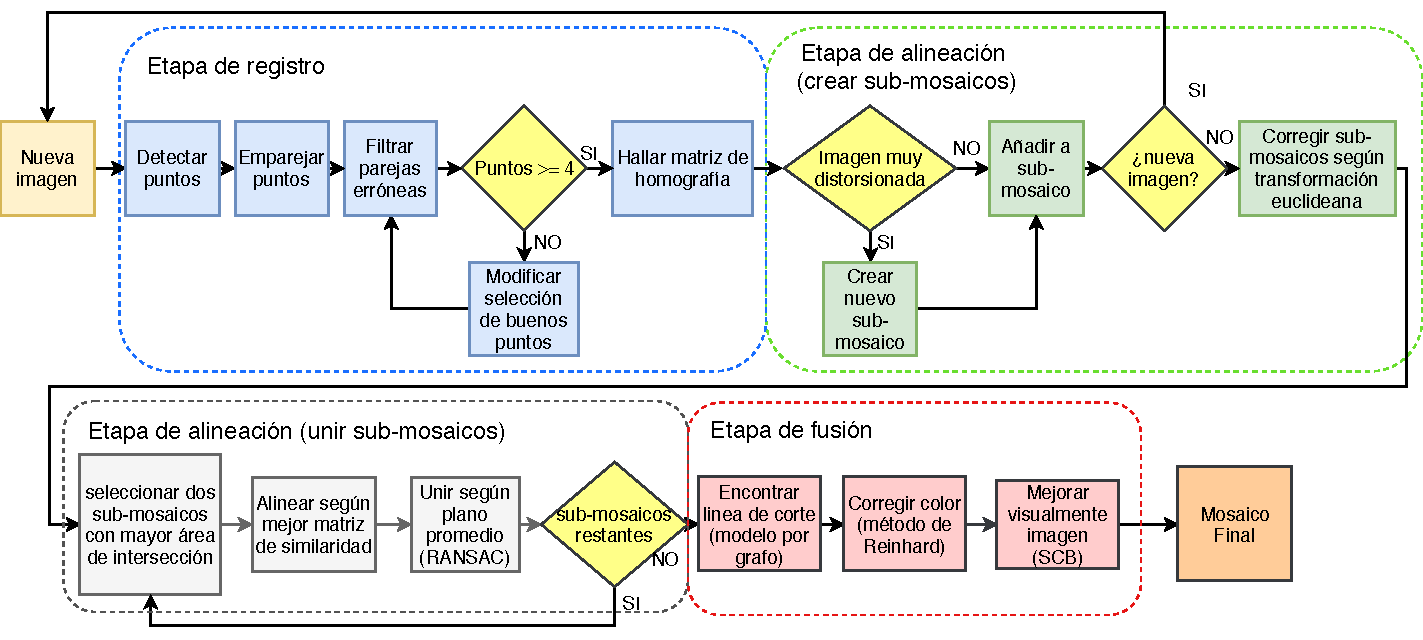
\includegraphics[width=1.21\textwidth]{esquema-general}}
		\caption{Esquema propuesto para la construcción del mosaico}
	
	\label{imagen:esquema}
\end{figure}

\section{OpenCV}